\chapter{Technology and method}
\lhead{\emph{Technology and method}}

\section{Introduction}
% Var vi limited til å følge matistikk?
In this chapter the technology and methods applied in this project is reasoned. After reading this chapter, one should be able to get a basic understanding of the approach and be able to reconstruct the results. The nature of the assignment required us to use tools which delivers high productivity and flexibility. 

\section{Technology} % syns denne kan eksistere fint her
When collaboration tools were chosen the focus was on finding the best tool for the situation. Tools should handle rapid changes, collaboration tools needs a low response time and stability. % Share\LaTeX for document processing and collaboration, Slack for team communication and Office365 as a shared storage service. These tools combined with git and github make a powerful combination which easily could have been swapped with some other tool.  % er skrevet under

\subsection{Version control}
Throughout this project git has been used as version control. The nature of the project made us choose Github. Github was chosen on the basis of it's well established, stable and it enables remote collaboration.

%\subsection{Collaboration tools}
%When collaboration tools were chosen the focus was on finding the best tool for the situation. Tools should handle rapid changes, collaboration tools needs a low response time and stability. % Share\LaTeX for document processing and collaboration, Slack for team communication and Office365 as a shared storage service. These tools combined with git and github make a powerful combination which easily could have been swapped with some other tool.  % er skrevet under

%\subsubsection{Writing}
\subsection{Collaboration tools}
\LaTeX \ was chosen as document preparation system. \LaTeX \ makes it simpler to generate professional looking papers. It also has good support for writing equations, creating figures, and can be extended with packages to expand its functionality. ShareLaTeX was used for real time collaboration in the same \LaTeX \ document. 

For storage and mail Office365 was used (OneDrive and Outlook), this is a tool provided by NTNU for it's students. This platform enables us to easily communicate with our product owners and mentor in addition to storing our project documents and attachments.


\subsection{Python and frameworks}
The choice of programming language was influenced mainly by its ability to integrate into already existing techonlogy, and the availability of machine learning tools. Python was a natural choice as the current application (Matistikk), was written in Django. TensorFlow, a popular machine learning library written by Google, also has bindings to Python. For machine learning, Keras\cite{chollet_keras_2015}, which is a higher level machine learning library with integration to TensorFlow, was chosen. Keras has excellent documentation and it's functionality makes it a delight to use. Keras is well suited for quick prototyping and it provides the engineer with the productivity needed to make a proof of concept as quickly as possible.


A client application was also needed to draw symbols, collect data and present statistics. To keep the application architecture simple, regular HTML, CSS and JavaScript with JQuery was chosen. Tornado was chosen to serve the HTML file and the API. Tornado is a simple framework to build web servers in Python and  was chosen because of its simplicity and the availability of WebSockets.
% HTML file and 'an or the' API ???

\section{Architecture}
The data used in this project is both sequential coordinates from CROHME (InkML example: \ref{lst:InkML_ex}) and image data. Because our data was sequential it became natural to use a WebSocket in the initial development phase. Both to resemble data format and to build ideas around how to keep all the information which lies within sequential coordinates. 
For the sake of simplicity, it was also implemented a way to do this over a simple http post request as an alternative to the WebSocket implementation. Doing it this way created a simple, but solid foundation for the engineers behind Matistikk to do it the way they wanted. \\
%After discussion with our project owners, we were drawn to the direction of using a http post request. The test application also does not think about the amount of data it sends per classification request. If the canvas is changed, it still re-sends the entire buffer. This is both to easy re-evaluate the buffer, but in addition this can trigger changes in the segmentation process, which can eventually lead to a different classification. % tror ikke denne trengs

\section{Preparing data}
This section will go through the process from when each symbol was segmented, to how the symbols were converted to input in the neural networks.

The data used as train data for the neural networks was in an XML format called InkML. In order to use this data as input to the neural networks, two main preprocessing steps were made. The data was first parsed, converted to NumPy arrays and normalized, then converted to images.

The data received from the front end application was processed in the same way, however without parsing the InkML files. Opposed to the data received from InkML, this data was not already segmented, and this process had to be completed first. The process for segmenting symbols is described in \ref{the_recognintion_system}.

The motivation for converting data to images was to use already existing models created for the MNIST dataset as a fundation for further work.

\subsection{Traces}
The coordinates received from InkML and the front end application included coordinates at different scales. Therefore the traces had to be scaled, where the chosen scale was within the range $[-1, 1]$, while still keeping the same proportions. The scaling process is described in \ref{scale_linear_by_column}.

An example of a trace received from InkML can be seen in \ref{fig:sqrt_not_processed}.
\begin{figure}[H]
    \centering
    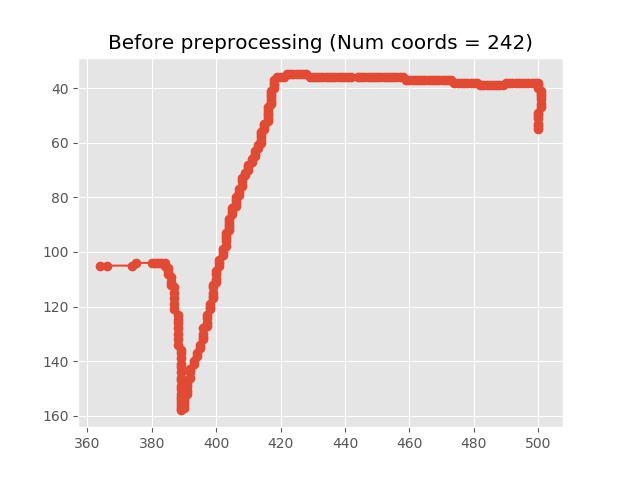
\includegraphics[width=\linewidth,keepaspectratio]{Assets/Chapter3_Method/sqrt_before_preprocessing.png}
    \caption{A square root which has not been through preprocessing.}
    \label{fig:sqrt_not_processed}
\end{figure}

The traces were recorded with different sampling frequencies. Some traces included several hundred points per symbol, while others included less than ten points per symbol. In order to improve performance of the networks, and make the input data normalized, the number of data points per symbol was reduced through a variant of the Ramer-Douglas-Peucker algorithm \ref{ramer_douglas_peucker}. All symbols' data points were reduced to a maximum of 40 data points. If the original tracing had less than 40 data points, it was padded using leading zeros. An example of the resulting trace which was used as input to the RNN model can be seen below.

\begin{figure}[H]
    \centering
    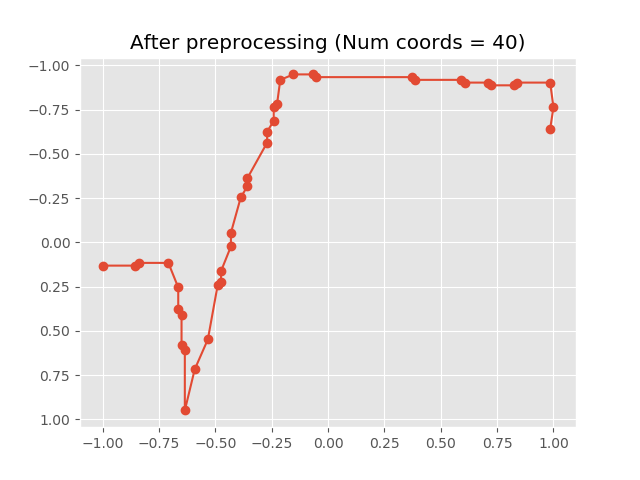
\includegraphics[width=\linewidth,keepaspectratio]{Assets/Chapter3_Method/sqrt_after_preprocessing.png}
    \caption{A square root after trace preprocessing.}
    \label{fig:sqrt_processed}
\end{figure}

\subsection{Images}

To prepare trace data for the convolutional neural network, the traces were converted into an image. In order to turn traces into images, the traces were first scaled by applying the the same scaling as previously \ref{scale_linear_by_column}, however within the range $[0, 26]$.

The next step was to generate an empty black image with 26x26 pixels (matrix of size 26x26 with only zeros). Afterwards, the pixels between each consecutive coordinate-pair were filled with white (255), and the resulting pixel grid was then normalized by dividing with 255. An example of the resulting grid presented as a matrix can be seen below, the example is simplified by using only a 8x10 matrix.

\begin{figure}[H]
    \begin{center}
    $
    \begin{bmatrix} % Jobbe mer forklaringen, vi scaler ikke 26x26 til 4x4 (?)
        \textcolor{gray}{0} & \textcolor{gray}{0} & \textcolor{gray}{0} & \textcolor{gray}{0} & \textcolor{gray}{0} & \textcolor{gray}{0} & \textcolor{gray}{0} & \textcolor{gray}{0} & \textcolor{gray}{0} & \textcolor{gray}{0} \\
        \textcolor{gray}{0} & \textcolor{gray}{0} & \textcolor{gray}{0} & \textcolor{gray}{0} & 1 & 1 & 1 & 1 & 1 & \textcolor{gray}{0} \\
        \textcolor{gray}{0} & \textcolor{gray}{0} & \textcolor{gray}{0} & 1 & \textcolor{gray}{0} & \textcolor{gray}{0} & \textcolor{gray}{0} & \textcolor{gray}{0} & \textcolor{gray}{0} & 1 \\
        1 & \textcolor{gray}{0} & \textcolor{gray}{0} & 1 & \textcolor{gray}{0} & \textcolor{gray}{0} & \textcolor{gray}{0} & \textcolor{gray}{0} & \textcolor{gray}{0} & \textcolor{gray}{0} \\
        \textcolor{gray}{0} & 1 & \textcolor{gray}{0} & 1 & \textcolor{gray}{0} & \textcolor{gray}{0} & \textcolor{gray}{0} & \textcolor{gray}{0} & \textcolor{gray}{0} & \textcolor{gray}{0} \\
        \textcolor{gray}{0} & 1 & \textcolor{gray}{0} & 1 & \textcolor{gray}{0} & \textcolor{gray}{0} & \textcolor{gray}{0} & \textcolor{gray}{0} & \textcolor{gray}{0} & \textcolor{gray}{0} \\
        \textcolor{gray}{0} & 1 & \textcolor{gray}{0} & 1 & \textcolor{gray}{0} & \textcolor{gray}{0} & \textcolor{gray}{0} & \textcolor{gray}{0} & \textcolor{gray}{0} & \textcolor{gray}{0} \\
        \textcolor{gray}{0} & \textcolor{gray}{0} & 1 & \textcolor{gray}{0} & \textcolor{gray}{0} & \textcolor{gray}{0} & \textcolor{gray}{0} & \textcolor{gray}{0} & \textcolor{gray}{0} & \textcolor{gray}{0} \\

    \end{bmatrix}
    $
    \end{center}
    \caption{An 8x10 matrix representing a pixel grid of a square root symbol.} % burde nok ha litt mer forklaring, TODO flytt forklaringen ovenfor ned i caption. (?)
    \label{fig:sqrt_matrix}
\end{figure}

\begin{figure}[H]
    \centering
    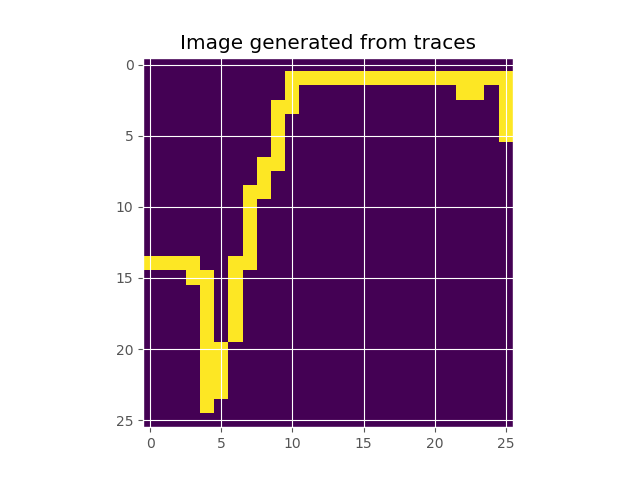
\includegraphics[width=\linewidth,keepaspectratio]{Assets/Chapter3_Method/sqrt_image.png}
    \caption{The resulting square root from the preprocessing done in previous steps.\\The generated image is 26x26 pixels.}
    \label{fig:sqrt_img}
\end{figure}

\section{The recognition system}
\label{the_recognintion_system}
The recognition system consists of both some "hard-coded" logic and the neural network. As stated in chapter \ref{handwriting_recognition}, handwriting recognition includes several steps required to classify correctly. The "hard-coded" logic solves the segmentation issue in an elementary way. The approach on the segmentation issue leaves the system vulnerable for noisy inputs. In addition, the system does a lot of preprocessing to make sure that the data flowing from the front end to the back end is roughly the same size, format, data type and so forth. 

[TODO] simple diagram of the whole process % vurder nødvendighet ?

\subsection{Preprocessing and segmentation}
%\section{Segmentation}
A large part of our approach relies on the segmentation of data, some symbols are put together by multiple traces, for example the number 4. Experimentation on finding the best solution for the segmentation issue led to object bounding boxes. Even though bounding boxes has potential to be the best solution for segmentation, it didn't perform as desired in terms of accuracy. In addition to it not proving to be as valuable as first thought we experienced good results with the previously mentioned "hard-coded" logic approach.

%The project went initially for a solution with a CNN, we had to separate the system into different tasks in order to make prediction. The reason behind this is that the CNN itself, in our solution should solely work on the classification of a symbol. Since our assignment is to handle symbols and expressions, we then need to extract single symbols from multiple symbols or expressions.\\
%This specific task was and is the most critical in order to get correct recognition with a CNN. If the segmentation turned out wrong, the classification would be handed bad data which makes a correct classification unlikely.\\ To solve the segmentation issue different approaches was attempted, among those were object localization and detection, with bounding boxes to easily detect symbols which consists of multiple strokes or traces. This idea of object detection was quite good and would have, if successful made the rest quite easy in comparison.\\ The attempts made on object detection was unsuccessful, we were getting results, but they were not proving to be better than solving it with a much simpler algorithm which did not require machine learning in the first place. 

[TODO] positional and proportional attributes assigned to the symbols


\subsection{Model architecture} % ?Classification | ?Models | ?Model architecture
Considering the lack of experience within the project participants, tutorials and articles needed to be read and understood. We quickly adapted and initially went after a solution with a CNN even though our primary data was sequential coordinates at that time. A recurrent network became more interesting after becoming more familiar with different use-cases and it's potential.

\textbf{TODO: Beskriv hva de ulike lagene er (dense = fully connected etc.)}

\subsubsection{RNN model}

The RNN model includes two one-dimensional convolution layers with max pooling and batch normalization. It also includes two bidirectional Gated Recurrent Unit layers. This model was first inspired by the Google Quick Draw model \cite{_recurrent_????}. It has been modified to correspond with the train dataset's input- and output data. The models architecture was also modified through experimentation to produce a better result on the test dataset.
\begin{figure}[H]
    \centering
    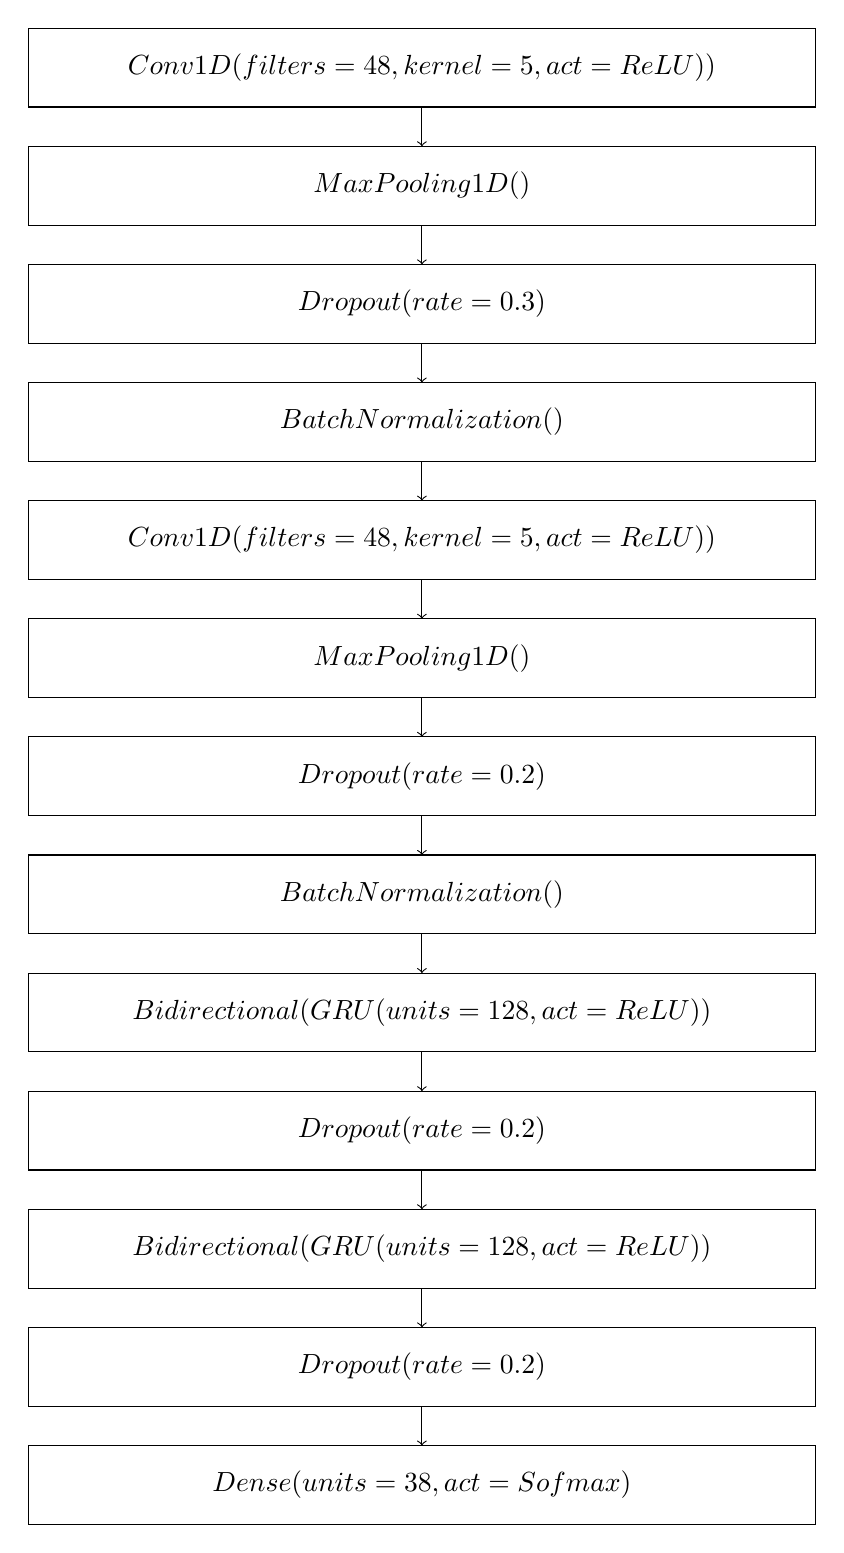
\begin{tikzpicture}
        \draw [black] (0, 1) rectangle (10, 0);
        \node[] at (5,0.5) {$Conv1D(filters=48, kernel=5, act=ReLU))$};
        \draw[->] (5, 0) -- (5, -0.5);
        
        \draw [black] (0, -0.5) rectangle (10, -1.5);
        \node[] at (5,0.-1) {$MaxPooling1D()$};
        \draw[->] (5, -1.5) -- (5, -2);

        \draw [black] (0, -2) rectangle (10, -3);
        \node[] at (5, -2.5) {$Dropout(rate=0.3)$};
        \draw[->] (5, -3) -- (5, -3.5);
        
        \draw [black] (0, -3.5) rectangle (10, -4.5);
        \node[] at (5, -4) {$BatchNormalization()$};
        \draw[->] (5, -4.5) -- (5, -5);
        
        \draw [black] (0, -5) rectangle (10, -6);
        \node[] at (5, -5.5) {$Conv1D(filters=48, kernel=5, act=ReLU))$};
        \draw[->] (5, -6) -- (5, -6.5);
        
        \draw [black] (0, -6.5) rectangle (10, -7.5);
        \node[] at (5, -7) {$MaxPooling1D()$};
        \draw[->] (5, -7.5) -- (5, -8);

        \draw [black] (0, -8) rectangle (10, -9);
        \node[] at (5, -8.5) {$Dropout(rate=0.2)$};
        \draw[->] (5, -9) -- (5, -9.5);
        
        \draw [black] (0, -9.5) rectangle (10, -10.5);
        \node[] at (5, -10) {$BatchNormalization()$};
        \draw[->] (5, -10.5) -- (5, -11);

        \draw [black] (0, -11) rectangle (10, -12);
        \node[] at (5, -11.5) {$Bidirectional(GRU(units=128, act=ReLU))$};
        \draw[->] (5, -12) -- (5, -12.5);

        \draw [black] (0, -12.5) rectangle (10, -13.5);
        \node[] at (5, -13) {$Dropout(rate=0.2)$};
        \draw[->] (5, -13.5) -- (5, -14);
        
        \draw [black] (0, -14) rectangle (10, -15);
        \node[] at (5, -14.5) {$Bidirectional(GRU(units=128, act=ReLU))$};
        \draw[->] (5, -15) -- (5, -15.5);
        
        \draw [black] (0, -15.5) rectangle (10, -16.5);
        \node[] at (5, -16) {$Dropout(rate=0.2)$};
        \draw[->] (5, -16.5) -- (5, -17);
        
        \draw [black] (0, -17) rectangle (10, -18);
        \node[] at (5, -17.5) {$Dense(units=38, act=Sofmax)$};


    \end{tikzpicture}
    \caption{A visualisation of the layer architecture in the RNN model.}
    \label{fig:RNN__model_visualization_1}
\end{figure}

\subsubsection{CNN model}

The CNN model has two convolution layers, a max pooling layer and two fully connected layers. The model had issues with overfitting, and it therefore includes two dropout layers with  rate of 25\% and 50\% respectively. The model also includes a flatten layer. The flatten layer performs a dimensionality reduction on the matrix returned from the convolutional layers. This model is inspired by CNN models with good results on the MNIST dataset. \textbf{TODO: Kilde for en paper med lignende arkitektur}
\begin{figure}[H]
    \centering
    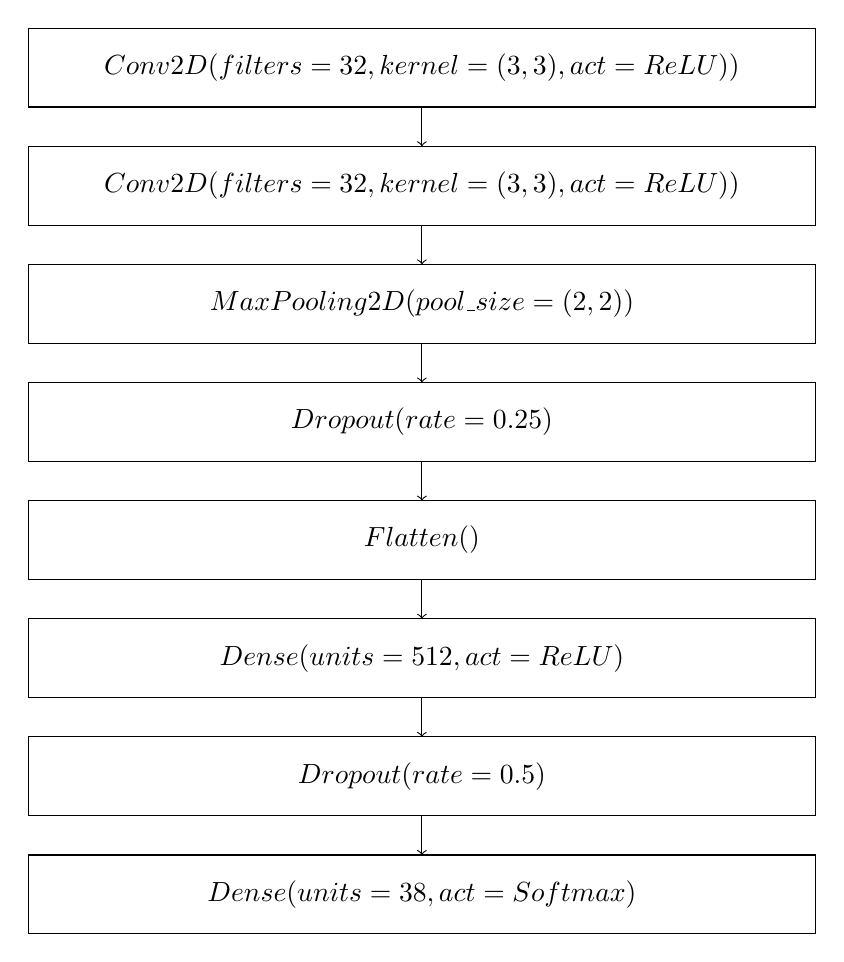
\begin{tikzpicture}
        \draw [black] (0, 1) rectangle (10, 0);
        \node[] at (5,0.5) {$Conv2D(filters=32, kernel=(3,3), act=ReLU))$};
        \draw[->] (5, 0) -- (5, -0.5);
        
        \draw [black] (0, -0.5) rectangle (10, -1.5);
        \node[] at (5,0.-1) {$Conv2D(filters=32, kernel=(3,3), act=ReLU))$};
        \draw[->] (5, -1.5) -- (5, -2);

        \draw [black] (0, -2) rectangle (10, -3);
        \node[] at (5, -2.5) {$MaxPooling2D(pool\_size=(2,2))$};
        \draw[->] (5, -3) -- (5, -3.5);
        
        \draw [black] (0, -3.5) rectangle (10, -4.5);
        \node[] at (5, -4) {$Dropout(rate=0.25)$};
        \draw[->] (5, -4.5) -- (5, -5);
        
        \draw [black] (0, -5) rectangle (10, -6);
        \node[] at (5, -5.5) {$Flatten()$};
        \draw[->] (5, -6) -- (5, -6.5);
        
        \draw [black] (0, -6.5) rectangle (10, -7.5);
        \node[] at (5, -7) {$Dense(units=512, act=ReLU)$};
        \draw[->] (5, -7.5) -- (5, -8);

        \draw [black] (0, -8) rectangle (10, -9);
        \node[] at (5, -8.5) {$Dropout(rate=0.5)$};
        \draw[->] (5, -9) -- (5, -9.5);
        
        \draw [black] (0, -9.5) rectangle (10, -10.5);
        \node[] at (5, -10) {$Dense(units=38, act=Softmax)$};

    \end{tikzpicture}
    \caption{A visualisation of the layer architecture in the CNN model.}
    \label{fig:RNN__model_visualization_2}
\end{figure}

\subsubsection{Combined model}

The combined model's architecture is a concatenation of the results from the CNN model, and the RNN model. The two models' last fully connected layer was removed before concatenation, to preserve as much information as possible. The combined model also has two fully connected layers and a dropout layer. The purpose of these layers is to enable the model to make its own predictions from the results of both input models.
\begin{figure}[H]
    \centering
    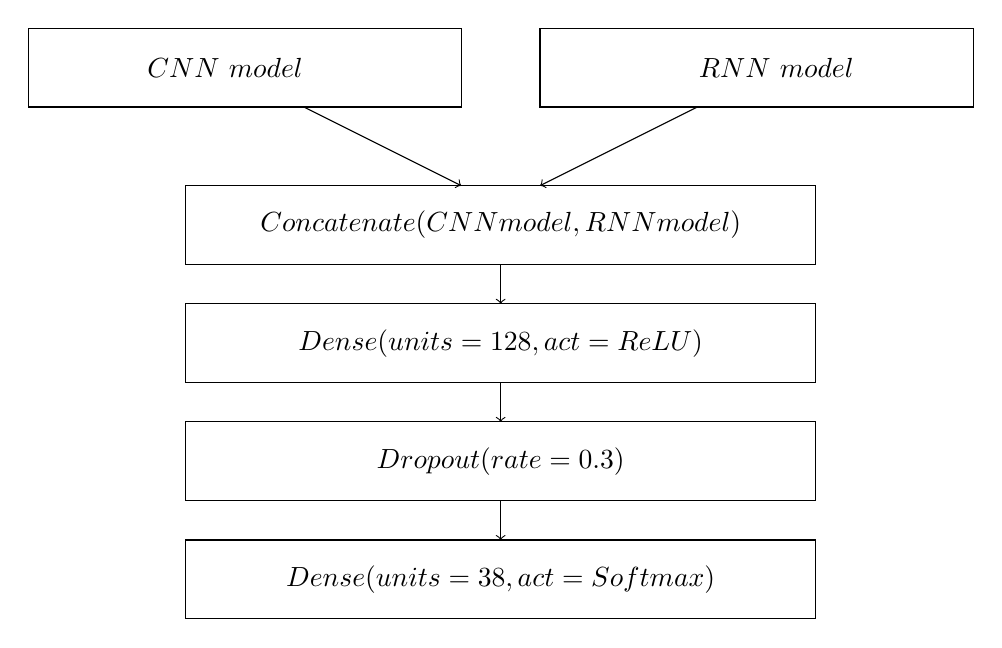
\begin{tikzpicture}
        \draw [black] (-6, -1) rectangle (-0.5, 0);
        \node[] at (-3.5,-0.5) {$CNN\ model$};
        \draw[[->] (-2.5, -1) -- (-0.5, -2);

        \draw [black] (0.5, -1) rectangle (6, 0);
        \node[] at (3.5,-0.5) {$RNN\ model$};
        \draw[[->] (2.5, -1) -- (0.5, -2);

        \draw [black] (-4, -2) rectangle (4, -3);
        \node[] at (0,-2.5) {$Concatenate(CNN model, RNN model)$};
        \draw[[->] (0, -3) -- (0, -3.5);
        
        \draw [black] (-4, -3.5) rectangle (4, -4.5);
        \node[] at (0,-4) {$Dense(units=128, act=ReLU)$};
        \draw[[->] (0, -4.5) -- (0, -5);
        
        \draw [black] (-4, -5) rectangle (4, -6);
        \node[] at (0,-5.5) {$Dropout(rate=0.3)$};
        \draw[[->] (0, -6) -- (0, -6.5);
        
        \draw [black] (-4, -6.5) rectangle (4, -7.5);
        \node[] at (0,-7) {$Dense(units=38, act=Softmax)$};

    \end{tikzpicture}
    \caption{A visualisation of the layer architecture in the combined model.}
    \label{fig:RNN__model_visualization_3}
\end{figure}
\subsection{Interpretation and context search}
%\section{Interpretation and context search} % SKRIVER LITT OM DETTE I \section{Segmentation}
% Har skrevet om at vi hardkodet segmentering, så ta det derfra. (fins i \section{Segmentation})

The interpretation system consist of a recursive search function and a set of fixed rules to determine the context of how the symbols fit together. This step receives a list of the classified symbols from the classification step as input and outputs the interpreted context in a tree based format of objects. This tree is sent back as a list of objects, where some of them links to other objects. % TODO review; er interpretation system rett ordbruk? 

\begin{figure}[H]
\begin{center}
    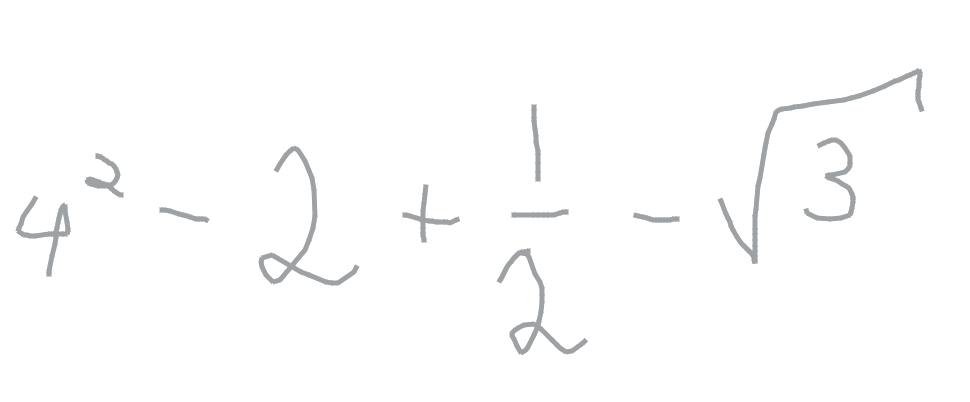
\includegraphics[scale=0.2]{Assets/Chapter3_Method/expression.png}
\end{center}
\centering
    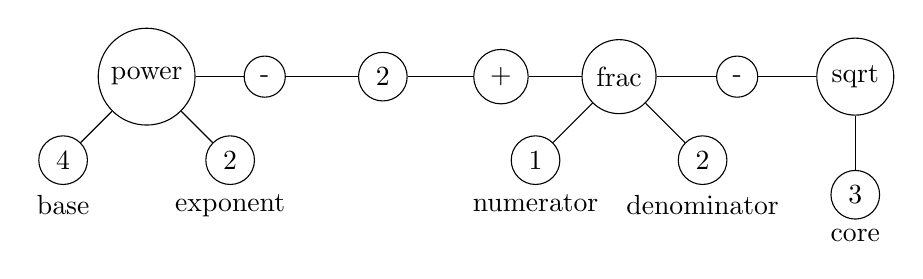
\begin{tikzpicture}[-,',auto,node distance=1.5cm,main node/.style={circle,draw}]
    \node[main node] (2) {power};
    \node[main node] (3) [right of=2] {-};
    \node[main node] (4) [right of=3] {2};
    \node[main node] (5) [right of=4] {+};
    \node[main node] (6) [right of=5] {frac};
    \node[main node] (7) [right of=6] {-};
    \node[main node] (8) [right of=7] {sqrt};
    
    \node[main node] (9) [below left of=2, label=below:base] {4};
    \node[main node] (10) [below right of=2, label=below:exponent] {2};
    
    \node[main node] (11) [below left of=6, label=below:numerator] {1};
    \node[main node] (12) [below right of=6, label=below:denominator] {2};
    
    \node[main node] (13) [below of=8, label=below:core] {3};
    
    

    \path[every node/.style={font=\sffamily\small}]
        (2) edge node [right] {} (3)
        (3) edge node [right] {} (4)
        (4) edge node [right] {} (5)
        (5) edge node [right] {} (6)
        (6) edge node [right] {} (7)
        (7) edge node [right] {} (8)
        (2) edge node [right] {} (9)
        (2) edge node [right] {} (10)
        (6) edge node [right] {} (11)
        (6) edge node [right] {} (12)
        (8) edge node [right] {} (13);

    \end{tikzpicture}
    \caption{An input expression and the resulting context tree.}

\label{fig:interpretation-tree1}
\end{figure}

% Dette kan kanskje legges i preprosessering et sted
%The symbols in the input list has a set of positional and proportional attributes that is used for sorting and to find all the symbols in an area. In addition, the attributes are used by the fixed rules to determine the notation used(see section frac-exp).


The system understands several mathematical notation elements, including square roots, fractions and exponents. Each of these elements has their own set of grammatical or positional rules that is used to find them (explained in section \ref{interpretation-square-roots} - \ref{interpretation-exponents}). In addition to these elements, some special symbols such as the equal sign and the multiplication dot is found and classified in this step (see section \ref{interpretation-special-symbols}).

\subsubsection{The main function}
% gangen i det hele
The main function in the interpretation system orchestrates the order of what element to search for. The order of elements searched for is:

\begin{enumerate}
    \setlength\itemsep{0.3em}
    \item Square roots
    \item Fractions
    \item Equal signs
    \item Multiplication dots
    \item Power groups, base and exponent
\end{enumerate}

The recursive part of this system comes from the square roots, fraction and exponents. If the body of a square root contains more than one symbol or object, the whole group is sent recursively to the main function. The same applies for the numerator and denominator found in fractions and for exponent-groups. The reason for this is to further search for context in these subgroups. For instance, fractions can have fractions as their numerator and exponents can consist of smaller expressions. 

This search process can be illustrated by a flowchart:

\begin{figure}[H]
\centering
    \begin{tikzpicture}[->,',auto,node distance=1.5cm,main node/.style={circle,draw},sub node/.style={draw}]
    \node[main node] (1) [label=above:Input] {};
    \node[sub node] (2) [below of=1] {Sqrt};
    \node[sub node] (3) [below of=2] {Frac};
    \node[sub node] (4) [below of=3] {$=$};
    \node[sub node] (5) [below of=4] {$\cdot$};
    \node[sub node] (6) [below of=5] {power};
    \node[main node] (7) [below of=6,label=below:Output] {};

    \path[every node/.style={font=\sffamily\small}]
        (1) edge node [right] {} (2)
        (2) edge node [right] {} (3)
        (3) edge node [right] {} (4)
        (4) edge node [right] {} (5)
        (5) edge node [right] {} (6)
        (6) edge node [right] {} (7)
        
        (2) edge[bend right=80] node [left] {core} (1)
        (3) edge[bend left=90] node [left] {numerator/denominator} (1)
        (6) edge[bend right=90] node [left] {exponent} (1);

    \end{tikzpicture}
    \caption{Flowchart of the order and recursion.}

\label{fig:interpretation_flowchart}
\end{figure}

To find the contents of a body (numerators, denominators, square roots), the interpretation system uses the positional values of the input symbols to check whether they are inside the bounds of an area or not. If their middle point is inside this area, they are added to the output group of the area search. This area is limited by a set of maximum and minimum x- and y-coordinates. These limits comes from a set of parameters required by the main function and the positional values of control units (square roots, fraction bars).

If a square root-, fraction- or exponent-element is found, the system creates an object of the correct type and links the relevant symbols to it. When creating one of these objects the traces for each of the input symbols are combined and new positional and proportional attributes are found.

Details about how these elements are found is described in the next sections.

\subsubsection{Square roots}
\label{interpretation-square-roots}
% detaljer om kvadratrot

The square root symbols are found by creating a list of all the input symbols classified as a square root sign, by filtering out all others. These are then sorted by width to make sure that the recursive logic is maintained when searching for the bodies. The widest one is most likely the outermost one if there are roots within roots. To find the bodies the system searches for objects within the bounds specified by the positional attributes of a square root. The widest square root is evaluated first.

\begin{figure}[H]
\centering
    \begin{tikzpicture}
        \node[anchor=south west,inner sep=0, scale=0.5] at (0,0) {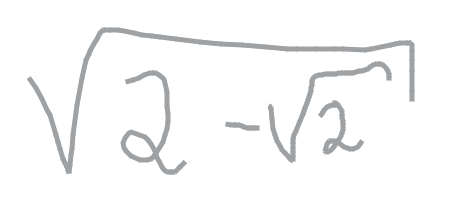
\includegraphics[width=\textwidth]{Assets/Chapter3_Method/interpretation-sqrt.png}};
        \draw[red, thick] (1.2,0.6) rectangle (6.7,2.8);
        \draw[blue, thick] (4.7,0.8) rectangle (6.3,2.3);
    \end{tikzpicture}
    \label{fig:interpretation}
\caption{Search area of square roots.}
\end{figure}

All the symbols and objects found inside are linked to the square root object as the body. This body is then sent recursively through the main function to find the context within the square root.

\begin{figure}[H]
\begin{center}
    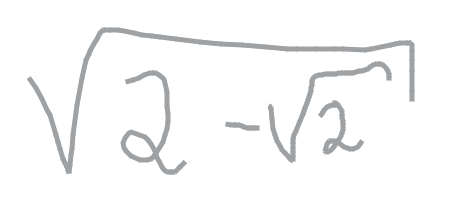
\includegraphics[scale=0.5]{Assets/Chapter3_Method/interpretation-sqrt.png}
\end{center}
\centering
    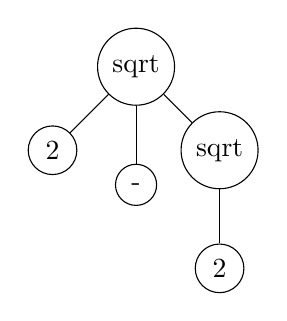
\begin{tikzpicture}[-,',auto,node distance=1.5cm,main node/.style={circle,draw}]
    \node[main node] (1) {sqrt};
    \node[main node] (2) [below left of=1] {2};
    \node[main node] (3) [below of=1] {-};
    \node[main node] (4) [below right of=1] {sqrt};
    \node[main node] (5) [below of=4] {2};

    \path[every node/.style={font=\sffamily\small}]
        (1) edge node [right] {} (2)
        (1) edge node [right] {} (3)
        (1) edge node [right] {} (4)
        (4) edge node [right] {} (5);

    \end{tikzpicture}
    \caption{An expression with a square root inside a square root and the resulting context tree.}

\label{fig:segmentation}
\end{figure}

\subsubsection{Fractions}

To find fractions the system searches for fraction bars by running the input symbols classified as minus signs through a test. To be classified as a fraction bar a minus sign must comply with one of the following cases:

\begin{itemize}
    \setlength\itemsep{0em}
    \item Have at least one symbol in the area over and under itself.
    \item Have at least two symbols in either the area over or the area under itself.
    \item Be the only minus sign in the input list and have at least one symbol in the area over or under itself.
\end{itemize}

To find the numerator and denominator of a fraction, the system searches for symbols in the area over and under the minus signs. The width of this area is specified by the leftmost and rightmost coordinate of the minus sign. The area never crosses the minus sign tested. The denominators and numerators found is also sent recursively through the main function to further look for context.

\begin{figure}[H]
\centering
\begin{tikzpicture}[-,',auto,node distance=1.5cm,main node/.style={circle,draw}]
    \node[anchor=south west,inner sep=0] (image) at (0,0) {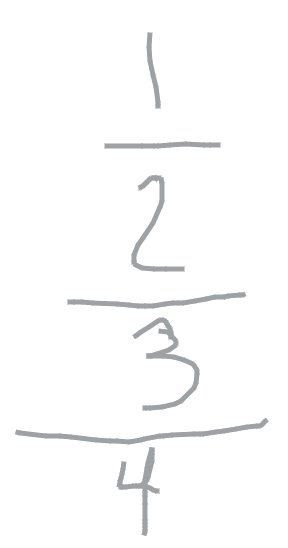
\includegraphics[width=0.2\textwidth]{Assets/Chapter3_Method/interpretation-frac.png}};
    
    \draw[red, thick] (0.2,0) rectangle (2.7,1.1);
    \draw[red, thick] (0.2,1.3) rectangle (2.7,6);
    \draw[blue, thick] (0.7,1.2) rectangle (2.5,2.5);
    \draw[blue, thick] (0.7,2.6) rectangle (2.5,6);
    \draw[purple, thick] (1.1,2.55) rectangle (2.2,4.1);
    \draw[purple, thick] (1.1,4.15) rectangle (2.2,6);
    
    \node [main node] (1) [right of=image, xshift=4cm, yshift=2cm]{frac};
    \node [main node] (2) [below left of=1]{frac};
    \node [main node] (3) [below right of=1]{4};
    \node [main node] (4) [below left of=2]{frac};
    \node [main node] (5) [below right of=2]{3};
    \node [main node] (6) [below left of=4]{1};
    \node [main node] (7) [below right of=4]{2};
    
    \node[rotate=45] (8) [below right of=5, xshift=-1cm, yshift=0.3cm]{denominators};
    \node[rotate=45] (9) [left of=2, xshift=0.5cm, yshift=1cm]{numerators};
    
    \path[every node/.style={font=\sffamily\small}]
        (1) edge node [right] {} (2)
        (1) edge node [right] {} (3)
        (2) edge node [right] {} (4)
        (2) edge node [right] {} (5)
        (4) edge node [right] {} (6)
        (4) edge node [right] {} (7);
\end{tikzpicture}
\caption{The search areas of a fraction expression with recursion and the corresponding context tree. The widest minus sign is considered the root fraction.}
\end{figure}

\subsubsection{Exponents}
\label{interpretation-exponents}

Exponents are found by checking if a pair of following symbols or objects forms a power-group. A power group is the object used for base/exponent groups. To form one of these groups the exponent has to be positioned such that the following rules are complied with:
\begin{itemize}
    \setlength\itemsep{0em}
    \item The lowest point of the exponent has to be higher up than the middle y-value of the base.
    \item The middle y value of the exponent has to higher up than the upper fourth of the base.
\end{itemize}
In addition, there is a special case rule if the exponent is an operator (-, +). Then, the lowest point of the exponent has to be higher up than the upper fourth of the base. The purpose of this is to increase the treshold to let a minus sign be the beginning of an exponent. Without this rule, expressions like '$2-2$' might mistakenly be recognized as '$2^{-}2$', since a minus sign is flat.

\begin{figure}[H]
\centering
\begin{tikzpicture}[-,',auto,node distance=1.5cm,main node/.style={circle,draw}]
    \node[anchor=south west,inner sep=0] (image) at (0,0) {
\includegraphics[width=0.2\textwidth]{Assets/Chapter3_Method/interpretation-exp.png}};
    \node[anchor=south west,inner sep=0] (image2) [left of=image, xshift=6cm] {
\includegraphics[width=0.2\textwidth]{Assets/Chapter3_Method/interpretation-exp.png}};
    
    \draw[-, red] (0,1.3) -- node[left, xshift=-2cm, yshift=-0.1cm] {middle point of base} (4,1.3);
    \draw[-, red] (0,1.65) -- node[left, xshift=-2cm, yshift=0.1cm] {lowest point of exp} (4,1.65);
    \draw[-, blue] (5,2.05) -- node[right, xshift=1.5cm, yshift=0.1cm] {middle point of exp} (8,2.05);
    \draw[-, blue] (5,1.7) -- node[right, xshift=1.5cm, yshift=-0.1cm] {top fourth of base} (8,1.7);
\end{tikzpicture}
\caption{Example of a power group and visualization of the first and second rule.}
\end{figure}

The system also supports groups of symbols and objects as base or exponent. Exponents within exponents is also supported. When a base and exponent is found, the system continues to check if the next symbol also is an exponent for the same base. This search continues until a symbol conflicts with one of the rules. All the found symbols is then sent recursively through the main function again.

\begin{figure}[H]
    \centering
    \begin{tikzpicture}[-,',auto,node distance=1.5cm,main node/.style={circle,draw}]
        \node[anchor=south west,inner sep=0] (image) at (0,0) {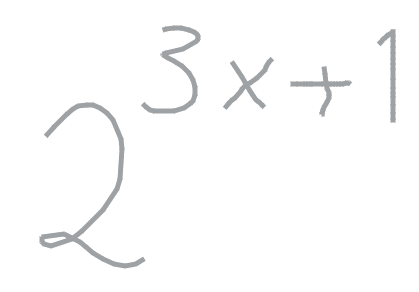
\includegraphics[width=0.2\textwidth]{Assets/Chapter3_Method/interpretation-exp2.png}};
    
        \node[anchor=south west,inner sep=0] (image2) [right of=image, xshift=4cm] {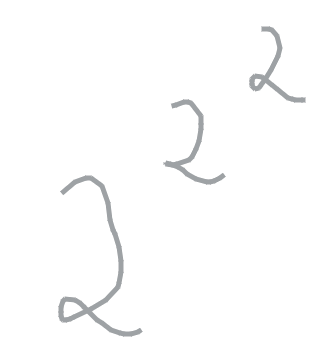
\includegraphics[width=0.2\textwidth]{Assets/Chapter3_Method/interpretation-exp3.png}};
        
        \node [main node] (1) [below of=image, yshift=-1.5cm]{power};
        \node [main node] (2) [below left of=1]{2};
        \node [main node] (3) [below right of=1]{group};
        \node [main node] (4) [below left of=3]{3};
        \node [main node] (5) [below of=3, xshift=-0.4cm]{x};
        \node [main node] (6) [below of=3, xshift=0.4cm]{+};
        \node [main node] (7) [below right of=3]{1};
        
        \node[rotate=0] (13) [left of=1, xshift=-0.2cm, yshift=-0.4cm]{Base};
        \node[rotate=0] (14) [right of=1, xshift=1cm, yshift=-0.4cm]{Exponent};
        
        \node [main node] (8) [below of=image2, yshift=-1.5cm]{power};
        \node [main node] (9) [below left of=8]{2};
        \node [main node] (10) [below right of=8]{power};
        \node [main node] (11) [below left of=10]{2};
        \node [main node] (12) [below right of=10]{2};
        
        \node[rotate=0] (15) [left of=11, xshift=0.5cm, yshift=0.4cm]{Bases};
        \node [] (16) [right of=10, xshift=0.4cm, yshift=-0.2cm]{Exponents};

        \path[every node/.style={font=\sffamily\small}]
            (1) edge node [right] {} (2)
            (1) edge node [right] {} (3)
            (3) edge node [right] {} (4)
            (3) edge node [right] {} (5)
            (3) edge node [right] {} (6)
            (3) edge node [right] {} (7)
            (8) edge node [right] {} (9)
            (8) edge node [right] {} (10)
            (10) edge node [right] {} (11)
            (10) edge node [right] {} (12);
            
    \end{tikzpicture}
    \caption{Power groups and their corresponding context tree.}
\end{figure}


\subsubsection{Special case symbols}
\label{interpretation-special-symbols}

In this system there are two special case symbols: the equal sign and the multiplication dot operator. These require special treatment due to how the segmentation and classification is done. An equal sign usually consist of two traces which would be interpreted as two minus signs since the segmentation step splits them up. The multiplication sign is a small dot that, when preprocessed and scaled up, would look similar to other round symbols like 0 and $\theta$. It would therefore most likely be misclassified.

To find equal signs the system searches for minus signs that are of similar size and lined up like an equal sign. To do this, each possible pair of minus signs in the input list is tested against some rules. The pair is classified as an equal sign only if these points are fulfilled:

\begin{itemize}
    \setlength\itemsep{0em}
    \item The width of the minus signs has to be similar. The difference in width has to be less than their average width.
    \item The difference between the center x-coordinate value has to be less than a third of their combined width.
    \item The difference between the center y-coordinate value has to be less than a their average width.
\end{itemize}

These rules became such after many rounds of testing. The idea behind them was to be as general as possible.

To find the multiplication signs the system searches for small symbols by looking at width, height and area. Symbols are classified as multiplication signs if these rules are fulfilled:

\begin{itemize}
    \setlength\itemsep{0em}
    \item The area (height*width) of the symbol has to be less than 250.
    \item Both the height and width has to be less than 20.
    \item The height and width has to be similar. One of them cannot be more than twice the other.
\end{itemize}

\subsection{Converting to \LaTeX}
After the context has been found, the results can be converted to the corresponding \LaTeX -code. For this, the truth values to all the output objects is combined in a string by a function. This function also has to be recursive, since the output objects might be fractions, square root or base-exponent groups. If a fraction is found, the contents of the numerator and denominator is sent through the same function. The same applies for the square root cores, exponents and bases.

\section{The project process} % 
The project process in terms of software engineering methodology had been a mix between multiple concepts and paradigms. Methodologies from the agile world were mostly used, such as tri programming. In the early stages of the project, we followed to some extent a methodology called Lean startup. Lean startup focuses on creating a minimal viable product, often referred to as \gls{MVP}. When the MVP was out, constructive discussions with the product owners about what they liked and what they did not like. At a stage the project split in different ways, we were continuously working on improving the product in different ways. The primary focus and goal was still to obtain the highest possible accuracy.

\section{Teamwork and roles} % 
The assignment was not a classical software engineering project, thus a clear structure was not defined. In the early stages of software development and prototyping we had a structure which was Even on front end, Torkil on back end and Håvard exploring CNNs. The distribution of roles changed according to what the sprint goals were and how they would be achieved. %This means that the structure used in the first sprint was not the same in the second sprint.
% tja, trenger strukturen å være med? den even frontend osv ??
% Si noe om hvordan vi fikk motivasjon til struktur=?
%Since the project is more of a research based project, it was not easy to define a simple structure as more common in software engineering projects. Although, a simple structure was created to get the MVP up, this was Even on front end, Torkil and Håvard on back end. \\ % TODO Fortsett dette, se MAL
%With the MVP up, the project quickly took principles from agile thoughts and methodologies, even though we could not plan an entire sprint to detail, we had a stand-up meeting, or quick recap of the progress and issues. This enabled a dynamic and flexible structure which led us to working together quite effective, when the project stagnated, we would quickly help each other out. When it came to exploring the potential behind RNN it was simply not easy to grasp how to approach this issue in order to classify correctly. This took one of the project engineers several weeks to get going and when the attempts were up for evaluation and the other project engineers understood the issue, a better solution and RNN was created. % Trenger kanskje ikke?

%\subsection{Methodology}
